%% Standalone figure for the Statistical Mechanics exercises (Quiz 1).
%% Build: pdflatex quiz1_ternary.tex  (or run build.sh in this folder)
\documentclass[11pt,tikz,border=2pt]{standalone}
\usepackage{amsmath,amssymb}
\usetikzlibrary{arrows.meta, positioning}
\begin{document}
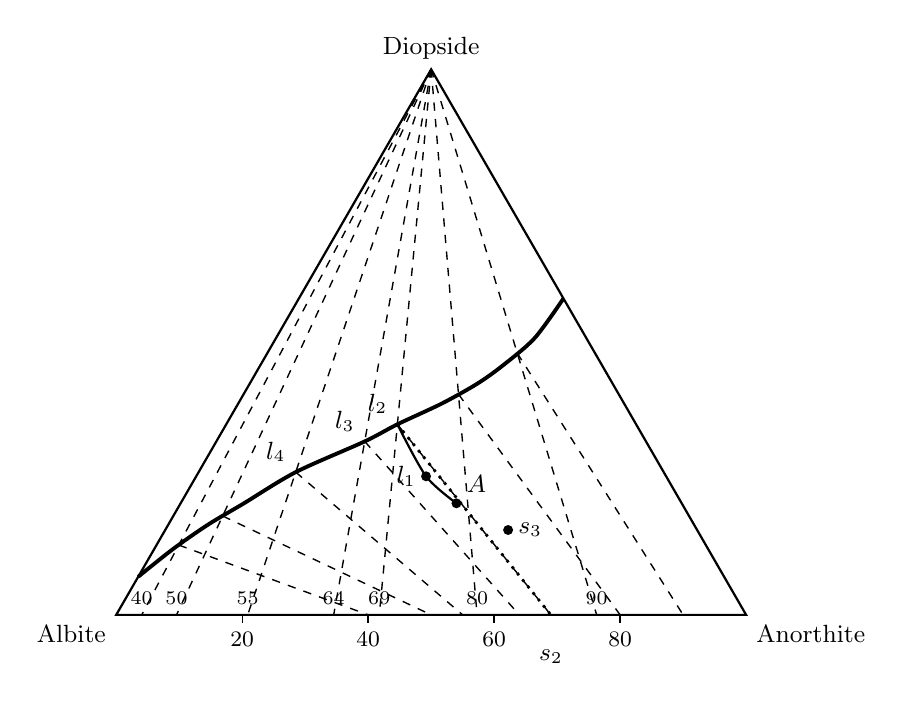
\begin{tikzpicture}[font=\small, >=Latex, line width=0.8pt]
    % corners and frame
    \coordinate (Ab) at (0,0);
    \coordinate (An) at (8,0);
    \coordinate (Di) at (4,6.928);
    \draw (Ab) -- (An) -- (Di) -- cycle;
    \node[below left] at (Ab) {Albite};
    \node[below right] at (An) {Anorthite};
    \node[above] at (Di) {Diopside};
    \foreach \p in {20,40,60,80}
        \draw[line width=0.5pt] (0.08*\p,0) -- (0.08*\p,-0.1) node[below, font=\footnotesize] {\p};
    % cotectic (boundary between the diopside and plagioclase fields)
    \draw[line width=1.4pt] plot[smooth] coordinates {(0.280,0.485) (0.728,0.841) (1.171,1.149) (1.614,1.412) (2.280,1.813) (3.156,2.203) (3.571,2.420) (4.135,2.684) (4.579,2.932) (4.903,3.162) (5.314,3.515) (5.680,4.018)};
    % diopside-liquid lines (from Di) and liquid-plagioclase tie lines;
    % numbers: An content of the plagioclase in equilibrium with each liquid
    \draw[dashed, line width=0.5pt] (Di) -- (0.794,0.887) -- (0.324,0.000);
    \draw[dashed, line width=0.5pt] (0.794,0.887) -- (3.200,0.000);
    \node[above, font=\scriptsize] at (0.324,0.000) {40};
    \draw[dashed, line width=0.5pt] (Di) -- (1.352,1.256) -- (0.766,-0.000);
    \draw[dashed, line width=0.5pt] (1.352,1.256) -- (4.000,0.000);
    \node[above, font=\scriptsize] at (0.766,-0.000) {50};
    \draw[dashed, line width=0.5pt] (Di) -- (2.280,1.813) -- (1.670,0.000);
    \draw[dashed, line width=0.5pt] (2.280,1.813) -- (4.400,0.000);
    \node[above, font=\scriptsize] at (1.670,0.000) {55};
    \draw[dashed, line width=0.5pt] (Di) -- (3.156,2.203) -- (2.762,0.000);
    \draw[dashed, line width=0.5pt] (3.156,2.203) -- (5.120,0.000);
    \node[above, font=\scriptsize] at (2.762,0.000) {64};
    \draw[dashed, line width=0.5pt] (Di) -- (3.571,2.420) -- (3.341,0.000);
    \draw[dashed, line width=0.5pt] (3.571,2.420) -- (5.520,0.000);
    \node[above, font=\scriptsize] at (3.341,0.000) {69};
    \draw[dashed, line width=0.5pt] (Di) -- (4.347,2.802) -- (4.583,0.000);
    \draw[dashed, line width=0.5pt] (4.347,2.802) -- (6.400,0.000);
    \node[above, font=\scriptsize] at (4.583,0.000) {80};
    \draw[dashed, line width=0.5pt] (Di) -- (5.093,3.325) -- (6.102,0.000);
    \draw[dashed, line width=0.5pt] (5.093,3.325) -- (7.200,0.000);
    \node[above, font=\scriptsize] at (6.102,0.000) {90};
    % crystallization of composition A
    \draw[dotted, line width=1pt] (3.571,2.420) -- (5.520,0.000);
    \draw plot[smooth] coordinates {(4.321,1.417) (3.935,1.760) (3.571,2.420)};
    \foreach \P/\n/\pos in {(4.321,1.417)/A/above right, (3.935,1.760)/l_1/left, (4.977,1.078)/s_3/right}
        { \fill \P circle (1.8pt); \node[\pos] at \P {$\n$}; }
    \node[above left] at (3.571,2.420) {$l_2$};
    \node[above left] at (3.156,2.203) {$l_3$};
    \node[above left] at (2.280,1.813) {$l_4$};
    \node[below=9pt] at (5.520,0.000) {$s_2$};
\end{tikzpicture}
\end{document}
